% TODO:
% http://www.usaco.org/index.php?page=viewproblem2&cpid=972
% https://codeforces.com/gym/102979/problem/G
% http://www.usaco.org/index.php?page=viewproblem2&cpid=698
% https://codeforces.com/contest/1146/problem/G
% https://codeforces.com/contest/1107/problem/E
% https://atcoder.jp/contests/arc104/tasks/arc104_f

\chapter{ম্যাট্রিক্স চেইন মাল্টিপ্লিকেশন এবং ইন্টারভাল ডিপি}

অধ্যায়ের টাইটেল দেখে হয়তো আন্দাজ করতে পারছো এই ধরনের ডিপিতে স্টেট হিসেবে একটা
অ্যারের সাব-অ্যারেকে ডিপিতে স্টেট হিসেবে রাখতে হবে। এই ক্যাটাগরির সবচাইতে
ক্লাসিক্যাল উদাহরণ দিয়ে শুরু করা যাক।

\section{একটি ক্লাসিক্যাল সমস্যা}

\begin{example}[ম্যাট্রিক্স চেইন মাল্টিপ্লিকেশন]
  $n (\le 500)$ টা ম্যাট্রিক্স আছে তোমার কাছে, তোমাকে সবচাইতে কম কস্টে তোমাকে
  এদের গুণফল বের করতে হবে। ফরমালি বলতে গেলে, তোমাকে $n$ টা ম্যাট্রিক্স $A_1,
  A_2,
  \ldots A_n$ এর dimension গুলো, অর্থাৎ, $(N_1, M_1), (N_2, M_2), \ldots,
  (N_n, M_n)$ গুলো দেওয়া আছে, যেখানে $A_i$ এর সাইজ হলো $n_i \times m_i$ আর,
  $M_i = N_{i+1} \, (1 \le i < n)$। তোমাকে বের করতে হবে সবচাইতে কম কতটি লুপ
  চালিয়ে তুমি $A_1 A_2 A_3 \dots A_n$ বের করতে পারবা। $a \times b$ এবং $b
  \times c$ সাইজের দুটি ম্যাটিক্স গুন করার কস্ট $abc$।
\end{example}

\begin{solution}
  তুমি যদি ম্যাট্রিক্স এক্সপোনেন্সিয়েশনের চ্যাপ্টারটি পড়ে থাকো তাহলে জানার
  কথা ম্যাট্রিক্স মাল্টিপ্লিকেশন একটি অ্যাসোসিয়েটিভ অপারেশন। যেমন, $(AB)C$ আর
  $A(BC)$ একই জিনিস, অর্থাৎ, $A$ আর $B$ এর গুণফল বের করে সেটাকে $C$ দিয়ে গুন
  দেওয়া যেই কথা, $A$ কে $B$ আর $C$ এর গুণফল দিয়ে গুন দেওয়াও একই কথা। কিন্তু
  এদের গুনের অর্ডারের উপর $ABC$ বের করতে কত টাইম লাগবে তা নির্ভর করে। যেমন
  ধরো, $A$, $B$ আর $C$ এর সাইজ যথাক্রমে $2 \times 1000$, $1000 \times 3$, $3
  \times 4$। যদি $(AB)C$ করি তাহলে কস্ট কত হয় দেখা যাক। প্রথমে $AB$
  করার জন্য কস্ট হলো $2 \times 1000 \times 3$, এবং এরপর $AB$ ম্যাট্রিক্সটির
  সাইজ হবে $2 \times 3$। এখন $(AB)$ এর সাথে $C$ গুন করার কস্ট হলো $2 \times 3
  \times 4$। সুতরাং মোট কস্ট হবে $2 \times 1000 \times 3 + 2 \times 3
  \times 4 = 6024$। কিন্তু $A(BC)$ এর ক্ষেত্রে কস্ট হবে $1000 \times 3 \times
  4 + 2 \times 1000 \times 4 = 20000$!

  একইভাবে ৪টা ম্যাট্রিক্সকে ৫ ভাবে, ৫টা ম্যাট্রিক্সকে ১৪ ভাবে গুন করতে পারবে।
  $n$ টা ম্যাট্রিক্সকে যতভাবে গুন করতে পারা যায় তাকে $C_{n-1}$ দিয়ে লেখা যায়,
  যেখানে $C_n$ হলো $n$-তম Catalan number। আসলে $n$ টা ম্যাট্রিক্স গুন করার
  প্রতিটা উপায়কেই আমরা একটা $n$ লিফের পারফেক্ট বাইনারি ট্রি\footnote{পারফেক্ট
  বাইনারি ট্রিঃ যেই রুটেড ট্রি এর লিফ ছাড়া প্রতিটা নোডের ২টা করে চাইল্ড আছে।
  } দিয়ে প্রকাশ করতে পারি। আর $n$ টা লিফের $C_{n-1}$ টা ভিন্ন ভিন্ন পারফেক্ট
  বাইনারি ট্রি আছে। $n$ তম Catalan number বের করার ফর্মুলা হলো $\frac{1}{n+1}
  \binom{2n}{n}$। চিত্র \ref{perfect_binary_trees_with_5_leaves}-তে ৫টা
  ম্যাট্রিক্স গুন করার সব উপায় দেখানো হয়েছে।
  \begin{figure}
    \centering
    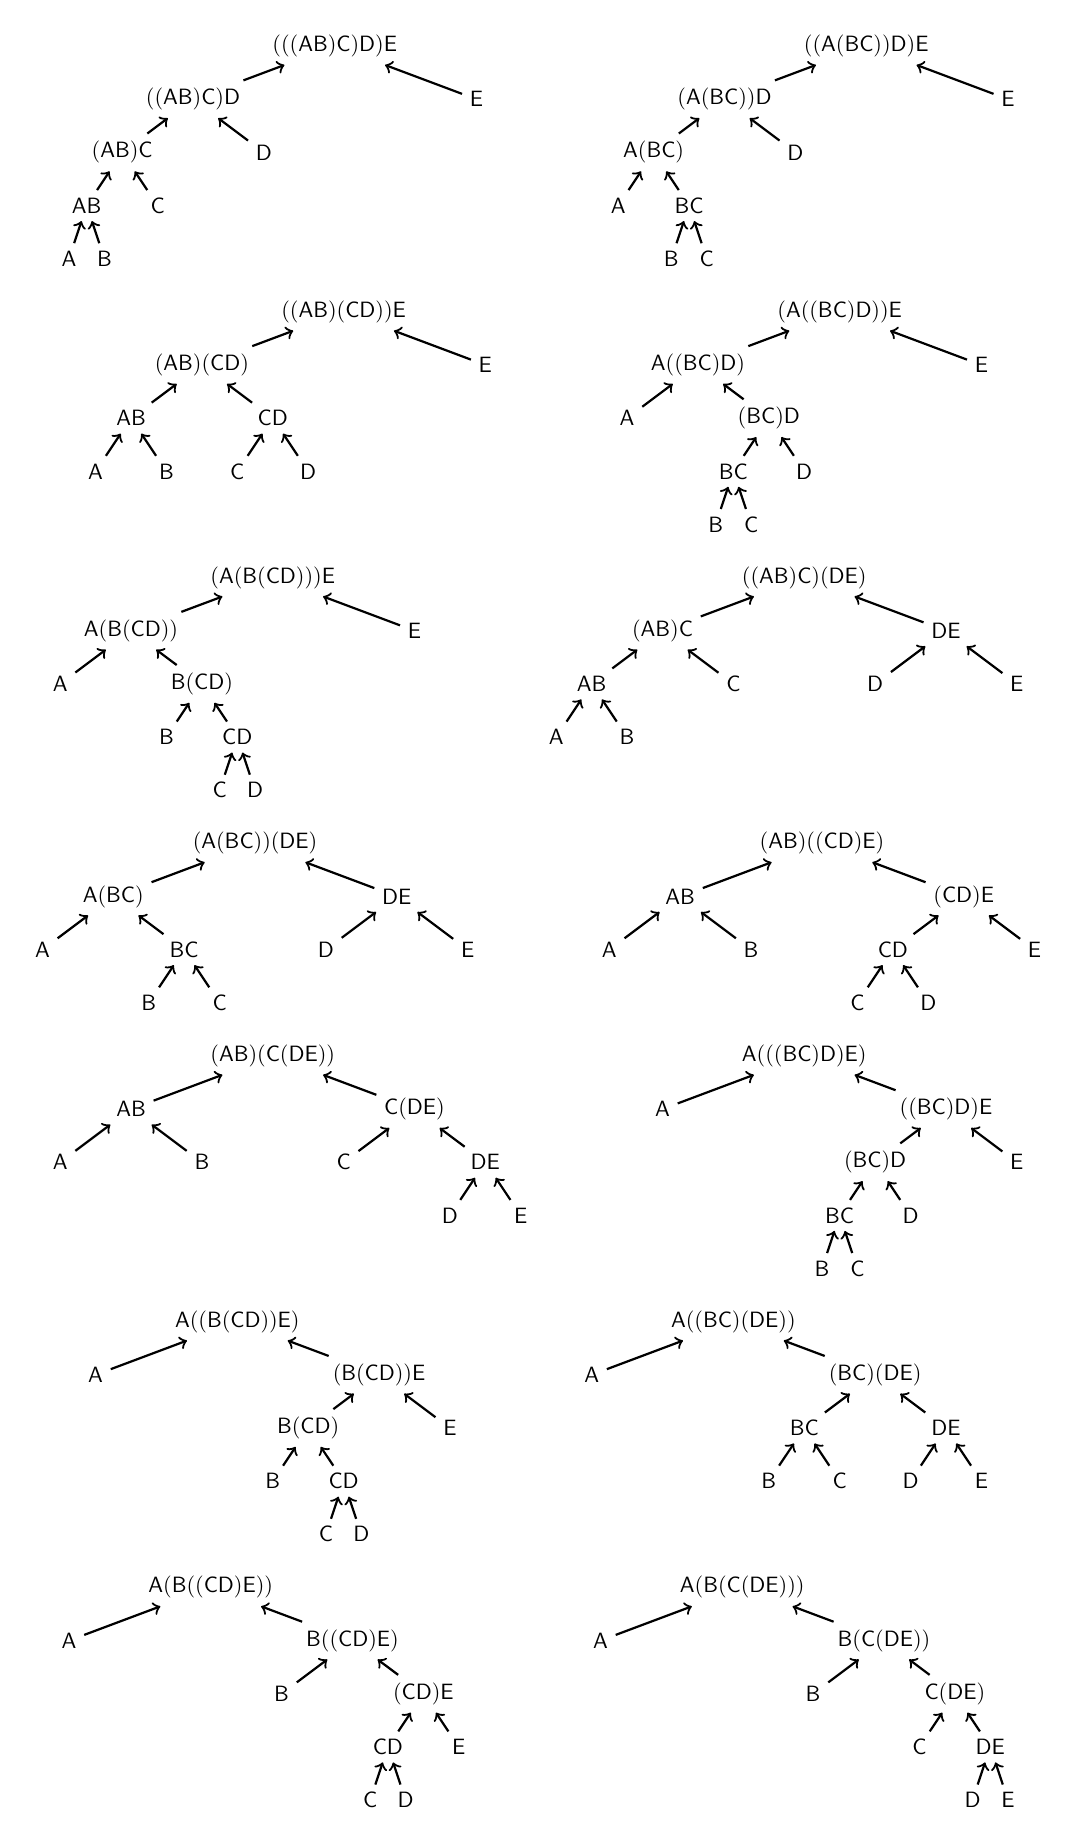
\begin{tikzpicture}[scale=0.9]
  \node[scale=0.8] (536) at (-6.625000,-2.750000) {$\mathsf{A}$};
  \node[scale=0.8] (537) at (-6.125000,-2.750000) {$\mathsf{B}$};
  \node[scale=0.8] (535) at (-6.375000,-2.000000) {$\mathsf{AB}$};
  \node[scale=0.8] (538) at (-5.375000,-2.000000) {$\mathsf{C}$};
  \node[scale=0.8] (534) at (-5.875000,-1.250000) {$\mathsf{(AB)C}$};
  \node[scale=0.8] (539) at (-3.875000,-1.250000) {$\mathsf{D}$};
  \node[scale=0.8] (533) at (-4.875000,-0.500000) {$\mathsf{((AB)C)D}$};
  \node[scale=0.8] (540) at (-0.875000,-0.500000) {$\mathsf{E}$};
  \node[scale=0.8] (532) at (-2.875000,0.250000) {$\mathsf{(((AB)C)D)E}$};
  \path[draw,thick,->] (536) -- (535);
  \path[draw,thick,->] (537) -- (535);
  \path[draw,thick,->] (535) -- (534);
  \path[draw,thick,->] (538) -- (534);
  \path[draw,thick,->] (534) -- (533);
  \path[draw,thick,->] (539) -- (533);
  \path[draw,thick,->] (533) -- (532);
  \path[draw,thick,->] (540) -- (532);
  \node[scale=0.8] (310) at (1.125000,-2.000000) {$\mathsf{A}$};
  \node[scale=0.8] (312) at (1.875000,-2.750000) {$\mathsf{B}$};
  \node[scale=0.8] (313) at (2.375000,-2.750000) {$\mathsf{C}$};
  \node[scale=0.8] (311) at (2.125000,-2.000000) {$\mathsf{BC}$};
  \node[scale=0.8] (309) at (1.625000,-1.250000) {$\mathsf{A(BC)}$};
  \node[scale=0.8] (314) at (3.625000,-1.250000) {$\mathsf{D}$};
  \node[scale=0.8] (308) at (2.625000,-0.500000) {$\mathsf{(A(BC))D}$};
  \node[scale=0.8] (315) at (6.625000,-0.500000) {$\mathsf{E}$};
  \node[scale=0.8] (307) at (4.625000,0.250000) {$\mathsf{((A(BC))D)E}$};
  \path[draw,thick,->] (312) -- (311);
  \path[draw,thick,->] (313) -- (311);
  \path[draw,thick,->] (310) -- (309);
  \path[draw,thick,->] (311) -- (309);
  \path[draw,thick,->] (309) -- (308);
  \path[draw,thick,->] (314) -- (308);
  \path[draw,thick,->] (308) -- (307);
  \path[draw,thick,->] (315) -- (307);
  \node[scale=0.8] (301) at (-6.250000,-5.750000) {$\mathsf{A}$};
  \node[scale=0.8] (302) at (-5.250000,-5.750000) {$\mathsf{B}$};
  \node[scale=0.8] (300) at (-5.750000,-5.000000) {$\mathsf{AB}$};
  \node[scale=0.8] (304) at (-4.250000,-5.750000) {$\mathsf{C}$};
  \node[scale=0.8] (305) at (-3.250000,-5.750000) {$\mathsf{D}$};
  \node[scale=0.8] (303) at (-3.750000,-5.000000) {$\mathsf{CD}$};
  \node[scale=0.8] (299) at (-4.750000,-4.250000) {$\mathsf{(AB)(CD)}$};
  \node[scale=0.8] (306) at (-0.750000,-4.250000) {$\mathsf{E}$};
  \node[scale=0.8] (298) at (-2.750000,-3.500000) {$\mathsf{((AB)(CD))E}$};
  \path[draw,thick,->] (301) -- (300);
  \path[draw,thick,->] (302) -- (300);
  \path[draw,thick,->] (304) -- (303);
  \path[draw,thick,->] (305) -- (303);
  \path[draw,thick,->] (300) -- (299);
  \path[draw,thick,->] (303) -- (299);
  \path[draw,thick,->] (299) -- (298);
  \path[draw,thick,->] (306) -- (298);
  \node[scale=0.8] (498) at (1.250000,-5.000000) {$\mathsf{A}$};
  \node[scale=0.8] (501) at (2.500000,-6.500000) {$\mathsf{B}$};
  \node[scale=0.8] (502) at (3.000000,-6.500000) {$\mathsf{C}$};
  \node[scale=0.8] (500) at (2.750000,-5.750000) {$\mathsf{BC}$};
  \node[scale=0.8] (503) at (3.750000,-5.750000) {$\mathsf{D}$};
  \node[scale=0.8] (499) at (3.250000,-5.000000) {$\mathsf{(BC)D}$};
  \node[scale=0.8] (497) at (2.250000,-4.250000) {$\mathsf{A((BC)D)}$};
  \node[scale=0.8] (504) at (6.250000,-4.250000) {$\mathsf{E}$};
  \node[scale=0.8] (496) at (4.250000,-3.500000) {$\mathsf{(A((BC)D))E}$};
  \path[draw,thick,->] (501) -- (500);
  \path[draw,thick,->] (502) -- (500);
  \path[draw,thick,->] (500) -- (499);
  \path[draw,thick,->] (503) -- (499);
  \path[draw,thick,->] (498) -- (497);
  \path[draw,thick,->] (499) -- (497);
  \path[draw,thick,->] (497) -- (496);
  \path[draw,thick,->] (504) -- (496);
  \node[scale=0.8] (516) at (-6.750000,-8.750000) {$\mathsf{A}$};
  \node[scale=0.8] (518) at (-5.250000,-9.500000) {$\mathsf{B}$};
  \node[scale=0.8] (520) at (-4.500000,-10.250000) {$\mathsf{C}$};
  \node[scale=0.8] (521) at (-4.000000,-10.250000) {$\mathsf{D}$};
  \node[scale=0.8] (519) at (-4.250000,-9.500000) {$\mathsf{CD}$};
  \node[scale=0.8] (517) at (-4.750000,-8.750000) {$\mathsf{B(CD)}$};
  \node[scale=0.8] (515) at (-5.750000,-8.000000) {$\mathsf{A(B(CD))}$};
  \node[scale=0.8] (522) at (-1.750000,-8.000000) {$\mathsf{E}$};
  \node[scale=0.8] (514) at (-3.750000,-7.250000) {$\mathsf{(A(B(CD)))E}$};
  \path[draw,thick,->] (520) -- (519);
  \path[draw,thick,->] (521) -- (519);
  \path[draw,thick,->] (518) -- (517);
  \path[draw,thick,->] (519) -- (517);
  \path[draw,thick,->] (516) -- (515);
  \path[draw,thick,->] (517) -- (515);
  \path[draw,thick,->] (515) -- (514);
  \path[draw,thick,->] (522) -- (514);
  \node[scale=0.8] (526) at (0.250000,-9.500000) {$\mathsf{A}$};
  \node[scale=0.8] (527) at (1.250000,-9.500000) {$\mathsf{B}$};
  \node[scale=0.8] (525) at (0.750000,-8.750000) {$\mathsf{AB}$};
  \node[scale=0.8] (528) at (2.750000,-8.750000) {$\mathsf{C}$};
  \node[scale=0.8] (524) at (1.750000,-8.000000) {$\mathsf{(AB)C}$};
  \node[scale=0.8] (530) at (4.750000,-8.750000) {$\mathsf{D}$};
  \node[scale=0.8] (531) at (6.750000,-8.750000) {$\mathsf{E}$};
  \node[scale=0.8] (529) at (5.750000,-8.000000) {$\mathsf{DE}$};
  \node[scale=0.8] (523) at (3.750000,-7.250000) {$\mathsf{((AB)C)(DE)}$};
  \path[draw,thick,->] (526) -- (525);
  \path[draw,thick,->] (527) -- (525);
  \path[draw,thick,->] (525) -- (524);
  \path[draw,thick,->] (528) -- (524);
  \path[draw,thick,->] (530) -- (529);
  \path[draw,thick,->] (531) -- (529);
  \path[draw,thick,->] (524) -- (523);
  \path[draw,thick,->] (529) -- (523);
  \node[scale=0.8] (489) at (-7.000000,-12.500000) {$\mathsf{A}$};
  \node[scale=0.8] (491) at (-5.500000,-13.250000) {$\mathsf{B}$};
  \node[scale=0.8] (492) at (-4.500000,-13.250000) {$\mathsf{C}$};
  \node[scale=0.8] (490) at (-5.000000,-12.500000) {$\mathsf{BC}$};
  \node[scale=0.8] (488) at (-6.000000,-11.750000) {$\mathsf{A(BC)}$};
  \node[scale=0.8] (494) at (-3.000000,-12.500000) {$\mathsf{D}$};
  \node[scale=0.8] (495) at (-1.000000,-12.500000) {$\mathsf{E}$};
  \node[scale=0.8] (493) at (-2.000000,-11.750000) {$\mathsf{DE}$};
  \node[scale=0.8] (487) at (-4.000000,-11.000000) {$\mathsf{(A(BC))(DE)}$};
  \path[draw,thick,->] (491) -- (490);
  \path[draw,thick,->] (492) -- (490);
  \path[draw,thick,->] (489) -- (488);
  \path[draw,thick,->] (490) -- (488);
  \path[draw,thick,->] (494) -- (493);
  \path[draw,thick,->] (495) -- (493);
  \path[draw,thick,->] (488) -- (487);
  \path[draw,thick,->] (493) -- (487);
  \node[scale=0.8] (471) at (1.000000,-12.500000) {$\mathsf{A}$};
  \node[scale=0.8] (472) at (3.000000,-12.500000) {$\mathsf{B}$};
  \node[scale=0.8] (470) at (2.000000,-11.750000) {$\mathsf{AB}$};
  \node[scale=0.8] (475) at (4.500000,-13.250000) {$\mathsf{C}$};
  \node[scale=0.8] (476) at (5.500000,-13.250000) {$\mathsf{D}$};
  \node[scale=0.8] (474) at (5.000000,-12.500000) {$\mathsf{CD}$};
  \node[scale=0.8] (477) at (7.000000,-12.500000) {$\mathsf{E}$};
  \node[scale=0.8] (473) at (6.000000,-11.750000) {$\mathsf{(CD)E}$};
  \node[scale=0.8] (469) at (4.000000,-11.000000) {$\mathsf{(AB)((CD)E)}$};
  \path[draw,thick,->] (471) -- (470);
  \path[draw,thick,->] (472) -- (470);
  \path[draw,thick,->] (475) -- (474);
  \path[draw,thick,->] (476) -- (474);
  \path[draw,thick,->] (474) -- (473);
  \path[draw,thick,->] (477) -- (473);
  \path[draw,thick,->] (470) -- (469);
  \path[draw,thick,->] (473) -- (469);
  \node[scale=0.8] (381) at (-6.750000,-15.500000) {$\mathsf{A}$};
  \node[scale=0.8] (382) at (-4.750000,-15.500000) {$\mathsf{B}$};
  \node[scale=0.8] (380) at (-5.750000,-14.750000) {$\mathsf{AB}$};
  \node[scale=0.8] (384) at (-2.750000,-15.500000) {$\mathsf{C}$};
  \node[scale=0.8] (386) at (-1.250000,-16.250000) {$\mathsf{D}$};
  \node[scale=0.8] (387) at (-0.250000,-16.250000) {$\mathsf{E}$};
  \node[scale=0.8] (385) at (-0.750000,-15.500000) {$\mathsf{DE}$};
  \node[scale=0.8] (383) at (-1.750000,-14.750000) {$\mathsf{C(DE)}$};
  \node[scale=0.8] (379) at (-3.750000,-14.000000) {$\mathsf{(AB)(C(DE))}$};
  \path[draw,thick,->] (381) -- (380);
  \path[draw,thick,->] (382) -- (380);
  \path[draw,thick,->] (386) -- (385);
  \path[draw,thick,->] (387) -- (385);
  \path[draw,thick,->] (384) -- (383);
  \path[draw,thick,->] (385) -- (383);
  \path[draw,thick,->] (380) -- (379);
  \path[draw,thick,->] (383) -- (379);
  \node[scale=0.8] (479) at (1.750000,-14.750000) {$\mathsf{A}$};
  \node[scale=0.8] (483) at (4.000000,-17.000000) {$\mathsf{B}$};
  \node[scale=0.8] (484) at (4.500000,-17.000000) {$\mathsf{C}$};
  \node[scale=0.8] (482) at (4.250000,-16.250000) {$\mathsf{BC}$};
  \node[scale=0.8] (485) at (5.250000,-16.250000) {$\mathsf{D}$};
  \node[scale=0.8] (481) at (4.750000,-15.500000) {$\mathsf{(BC)D}$};
  \node[scale=0.8] (486) at (6.750000,-15.500000) {$\mathsf{E}$};
  \node[scale=0.8] (480) at (5.750000,-14.750000) {$\mathsf{((BC)D)E}$};
  \node[scale=0.8] (478) at (3.750000,-14.000000) {$\mathsf{A(((BC)D)E)}$};
  \path[draw,thick,->] (483) -- (482);
  \path[draw,thick,->] (484) -- (482);
  \path[draw,thick,->] (482) -- (481);
  \path[draw,thick,->] (485) -- (481);
  \path[draw,thick,->] (481) -- (480);
  \path[draw,thick,->] (486) -- (480);
  \path[draw,thick,->] (479) -- (478);
  \path[draw,thick,->] (480) -- (478);
  \node[scale=0.8] (398) at (-6.250000,-18.500000) {$\mathsf{A}$};
  \node[scale=0.8] (401) at (-3.750000,-20.000000) {$\mathsf{B}$};
  \node[scale=0.8] (403) at (-3.000000,-20.750000) {$\mathsf{C}$};
  \node[scale=0.8] (404) at (-2.500000,-20.750000) {$\mathsf{D}$};
  \node[scale=0.8] (402) at (-2.750000,-20.000000) {$\mathsf{CD}$};
  \node[scale=0.8] (400) at (-3.250000,-19.250000) {$\mathsf{B(CD)}$};
  \node[scale=0.8] (405) at (-1.250000,-19.250000) {$\mathsf{E}$};
  \node[scale=0.8] (399) at (-2.250000,-18.500000) {$\mathsf{(B(CD))E}$};
  \node[scale=0.8] (397) at (-4.250000,-17.750000) {$\mathsf{A((B(CD))E)}$};
  \path[draw,thick,->] (403) -- (402);
  \path[draw,thick,->] (404) -- (402);
  \path[draw,thick,->] (401) -- (400);
  \path[draw,thick,->] (402) -- (400);
  \path[draw,thick,->] (400) -- (399);
  \path[draw,thick,->] (405) -- (399);
  \path[draw,thick,->] (398) -- (397);
  \path[draw,thick,->] (399) -- (397);
  \node[scale=0.8] (281) at (0.750000,-18.500000) {$\mathsf{A}$};
  \node[scale=0.8] (284) at (3.250000,-20.000000) {$\mathsf{B}$};
  \node[scale=0.8] (285) at (4.250000,-20.000000) {$\mathsf{C}$};
  \node[scale=0.8] (283) at (3.750000,-19.250000) {$\mathsf{BC}$};
  \node[scale=0.8] (287) at (5.250000,-20.000000) {$\mathsf{D}$};
  \node[scale=0.8] (288) at (6.250000,-20.000000) {$\mathsf{E}$};
  \node[scale=0.8] (286) at (5.750000,-19.250000) {$\mathsf{DE}$};
  \node[scale=0.8] (282) at (4.750000,-18.500000) {$\mathsf{(BC)(DE)}$};
  \node[scale=0.8] (280) at (2.750000,-17.750000) {$\mathsf{A((BC)(DE))}$};
  \path[draw,thick,->] (284) -- (283);
  \path[draw,thick,->] (285) -- (283);
  \path[draw,thick,->] (287) -- (286);
  \path[draw,thick,->] (288) -- (286);
  \path[draw,thick,->] (283) -- (282);
  \path[draw,thick,->] (286) -- (282);
  \path[draw,thick,->] (281) -- (280);
  \path[draw,thick,->] (282) -- (280);
  \node[scale=0.8] (506) at (-6.625000,-22.250000) {$\mathsf{A}$};
  \node[scale=0.8] (508) at (-3.625000,-23.000000) {$\mathsf{B}$};
  \node[scale=0.8] (511) at (-2.375000,-24.500000) {$\mathsf{C}$};
  \node[scale=0.8] (512) at (-1.875000,-24.500000) {$\mathsf{D}$};
  \node[scale=0.8] (510) at (-2.125000,-23.750000) {$\mathsf{CD}$};
  \node[scale=0.8] (513) at (-1.125000,-23.750000) {$\mathsf{E}$};
  \node[scale=0.8] (509) at (-1.625000,-23.000000) {$\mathsf{(CD)E}$};
  \node[scale=0.8] (507) at (-2.625000,-22.250000) {$\mathsf{B((CD)E)}$};
  \node[scale=0.8] (505) at (-4.625000,-21.500000) {$\mathsf{A(B((CD)E))}$};
  \path[draw,thick,->] (511) -- (510);
  \path[draw,thick,->] (512) -- (510);
  \path[draw,thick,->] (510) -- (509);
  \path[draw,thick,->] (513) -- (509);
  \path[draw,thick,->] (508) -- (507);
  \path[draw,thick,->] (509) -- (507);
  \path[draw,thick,->] (506) -- (505);
  \path[draw,thick,->] (507) -- (505);
  \node[scale=0.8] (209) at (0.875000,-22.250000) {$\mathsf{A}$};
  \node[scale=0.8] (211) at (3.875000,-23.000000) {$\mathsf{B}$};
  \node[scale=0.8] (213) at (5.375000,-23.750000) {$\mathsf{C}$};
  \node[scale=0.8] (215) at (6.125000,-24.500000) {$\mathsf{D}$};
  \node[scale=0.8] (216) at (6.625000,-24.500000) {$\mathsf{E}$};
  \node[scale=0.8] (214) at (6.375000,-23.750000) {$\mathsf{DE}$};
  \node[scale=0.8] (212) at (5.875000,-23.000000) {$\mathsf{C(DE)}$};
  \node[scale=0.8] (210) at (4.875000,-22.250000) {$\mathsf{B(C(DE))}$};
  \node[scale=0.8] (208) at (2.875000,-21.500000) {$\mathsf{A(B(C(DE)))}$};
  \path[draw,thick,->] (215) -- (214);
  \path[draw,thick,->] (216) -- (214);
  \path[draw,thick,->] (213) -- (212);
  \path[draw,thick,->] (214) -- (212);
  \path[draw,thick,->] (211) -- (210);
  \path[draw,thick,->] (212) -- (210);
  \path[draw,thick,->] (209) -- (208);
  \path[draw,thick,->] (210) -- (208);
\end{tikzpicture}

    \caption{৫টা ম্যাট্রিক্সকে গুন করার সবরকম উপায়}
    \label{perfect_binary_trees_with_5_leaves}
  \end{figure}

  ডায়াগ্রামটা যদি একটু ভালোমত দেখো তাহলে খেয়াল করবা আমরা প্রতিটা উপায় জেনারেট
  করার জন্য প্রথমে $ABCDE$ এর মঝে কোন এক জায়গায় ভাগ করেছি, ধরো $B$ আর $C$ এর
  মাঝে ভাগ করলাম, তারপর $AB$ এবং $CDE$ কে যতভাবে গুন করা যায় তা রিকারসিভলি
  হিসাব করেছি। আর এরপর $(AB)$ কে $(CDE)$ এর সাথে গুণ করার জন্য বিবেচনা করেছি।

  সুতরাং আমাদের ডিপি দেখতে এরকম হবেঃ $\DP \two{l}{r} = $ $A_l A_{l+1} A_{l+2}
  \dots A_{r}$ বের করার মিনিমাম কস্ট। বেস কেইসের জন্য $\DP \two{i}{i} = 0$,
  কারণ একটা ম্যাট্রিক্সের গুণফল বের করতে তো কোন অপারেশনই লাগে না। এখন, $l$
  থেকে $r$ ম্যাট্রিক্স গুলোর গুণফল বের করার জন্য আমরা মাঝখানে কোথাও, ধরি $i$
  আর $i+1$ তম ম্যাট্রিক্সের মাঝে ভাগ করলাম, তাহলে আমরা প্রথমে $A_l \dots A_i$
  আর $A_{i+1} \dots A_{r}$ বের করার অপ্টিমাল কস্ট হিসাব করবো, যেটা আমরা
  পাচ্ছি $\DP\two{l}{i}$ এবং $\DP\two{i+1}{r}$ তে। সাথে $(A_l \dots A_{i})
  \times (A_{i+1} \dots A_{r})$ করার কস্ট হলো $N_l M_i M_r$, কারণ $(A_l \dots
  A_{i})$ ম্যাট্রিক্সের এর সাইজ হবে $N_l \times M_i$ আর $(A_{i+1} \dots A_r)$
  ম্যাট্রিক্সের সাইজ হবে $N_{i+1} \times M_r$। সুতরাং $l < r$ এর ক্ষেত্রে
  ডিপির রিকারেন্স হলোঃ
  \[
    \DP\two{l}{r} = \min_{l \le i < r} \DP\two{l}{i} + \DP\two{i+1}{r} + N_l
    M_i M_r
  \]
  ফাইনাল অ্যান্সার হবে $\DP\two{1}{n}$।
\end{solution}

\begin{example}[\href{https://www.spoj.com/problems/MIXTURES/}{SPOJ -
  Mixtures}]
  হ্যারি পটারের সামনে পাশাপাশি একটা সারিতে $n \, (\le 100)$ টা মিশ্রণ সাজানো
  আছে। প্রত্যেকটা মিশ্রণের ১০০টা রঙের মধ্যে একটা রঙ আছে (০ থেক ৯৯ পর্যন্ত
  নাম্বারিং করা), $i$-তম মিশ্রণের রঙ $a_i \, (0 \le a_i \le 99)$। সে সবগুলা
  মিশ্রণকে একসাথে মিশানোর জন্য $n-1$ বার এই অপারেশনটি করবেঃ
  \begin{itemize}
    \item পাশাপাশি ২টা মিশ্রণ নিয়ে তাদের একসাথে মিশিয়ে ২টার মাঝখানে মিশ্রণটা
    রেখে দিবে, অর্থাৎ, বাকি মিশ্রণ গুলোর ক্রমের কোন পরিবর্তন হবে না। পাশাপাশি
    নির্বাচন করা মিশ্রণগুলোর রঙ যদি $x$ এবং $y$ হয়, তাহলে তাদের মিশ্রণের রঙ
    হবে $(x+y) \mod 100$\footnote{এখানে $a \mod m$ দিয়ে $a$ কে $m$ দিয়ে ভাগ
    করলে যেই ভাগশেষ থাকে তা বুঝানো হচ্ছে।}। আর তাদের মিশ্রিত করার সময় $xy$
    পরিমাণের ধোঁয়া উৎপন্ন হয়।
  \end{itemize}
  তোমাকে বের করতে হবে সবচাইতে কম কতো পরিমাণের ধোঁয়া উৎপন্ন করে মিশ্রণ গুলোকে
  হ্যারি মিশ্রিত করতে পারবে।
\end{example}

\begin{solution}
  আগের প্রবলেমের মতই এই প্রবলেমেও $n$টা মিশ্রণকে মিক্স করার যেকোনো উপায়কেই
  তুমি একটা $n$ লিফের পারফেক্ট বাইনারি ট্রি হিসেবে আঁকতে পারবা।
  $\DP\two{l}{r}$ হলো $l$ থেকে $r$ এর মধ্যে মিশ্রণ গুলোকে যদি অপ্টিমালি
  মিশানো হয়, তাহলে সর্বনিম্ন কি পরিমাণের ধোঁয়া উৎপন্ন হবে। এখন তুমি মাঝখানে
  কোথায় ভাঙ্গবে তার উপর ইটারেট করবা। ধরো, $i$ আর $i+1$ এর মাঝে ভাঙ্গেছো,
  তাহলে ২ পাশের কস্ট হলো $\DP\two{l}{i}$ আর $\DP\two{i+1}{r}$। $l \ldots i$
  এর মিশ্রণগুলোকে মিক্স করে যেই মিশ্রণ পাবো তার রঙ হবে $\left(\sum_{j=l}^{i}
  a_j \right) \mod 100$ (কারণ, $(((x+y)\mod m) + z) \mod m = (x+y+z) \mod
  m$)। একইভাবে $i+1 \ldots r$ এর মিশ্রণগুলোকে মিক্স করার পর $\left(
  \sum_{j=i+1}^{r} a_j \right) \mod 100$ রঙের মিশ্রণ পাবা। এদের মিক্স করলে
  আবার $\left( \left(\sum_{j=l}^{i} a_j \right) \mod 100 \right) \times
  \left( \left( \sum_{j=i+1}^{r} a_j \right) \mod 100 \right)$ পরিমাণের ধোঁয়া
  উৎপন্ন হবে। তাহলে রিকারেন্সটা হলোঃ
  \[
    \DP\two{l}{r} = \min_{i=l}^{r-1} \DP\two{l}{i} + \DP\two{i+1}{r} + L
    \times R
  \]
  যেখানে, $L = \left(\sum_{j=l}^{i} a_j \right) \mod 100$, $R = \left(
  \sum_{j=i+1}^{r} a_j \right) \mod 100$, এবং $\DP\two{i}{i} = 0$।
\end{solution}

\begin{example}[\href{http://www.usaco.org/index.php?page=viewproblem2&%
  cpid=972}{USACO - Greedy Pie Eaters}]
  ফার্মার জনের কাছে $M$টা গরু আর $N$ টা পাই আছে। গরুগুলো $1$ থেকে $M$ এবং
  পাইগুলো $1$ থেকে $N$ পর্যন্ত নাম্বারিং করা। $i$-তম গরু $[l_i, r_i]$ রেঞ্জের
  মধ্যে পাইগুলো খেতে পছন্দ করে। তোমাকে আরেকটা জিনিস বলে দেওয়া আছে, তা হলো ২টা
  গরুর পছন্দের রেঞ্জ একই হবে না কখনো। $i$-তম গরুর ওজন হলো $w_i$।

  \noindent ফার্মার জন একটা সিকুয়েন্স $c_1, c_2, \ldots, c_K$ বাছাই করবে,
  যেটা দিয়ে গরুগুলো কি অর্ডারে পাই খেতে আসবে তা বুঝাবে, অর্থাৎ, প্রথমে
  $c_1$-তম গরুটি আসবে, এরপর $c_2$-তম গরুটি আসবে...। একটা গরু আসলে সে তার
  পছন্দের রেঞ্জে বাকি থাকা সব পাই খেয়ে ফেলবে। কিন্তু যদি তার পছন্দের রেঞ্জে
  কোন পাইই বাকি না থাকে তাহলে সে মন খারাপ করে বসবে! ফার্মার জন এমন একটা
  সিকুয়েন্স বাছাই করতে চায় যাতে $(w_{c_1} + w_{c_2} + \ldots + w_{c_K})$ এর
  মান ম্যাক্সিমাইজ হয়, এবং বাছাই করা $K$ টা গরুর মধ্যে কেও মন খারাপ না করে।
  $1 \le N \le 300, 1 \le M \le \frac{N(N+1)}{2}, 1 \le w_i \le 10^6$।
\end{example}

\begin{solution}
  প্রবলেমটা সল্ভ করার জন্য প্রসেসটাতে কি হচ্ছে তা উলটা দিক থেকে চিন্তা করবো
  -- ধরো তুমি একটা সিকুয়েন্স $c_1, c_2, \ldots, c_K$ ঠিক করেছ। এখন এই
  সিকুন্সটা ভ্যালিড হতে হলে প্রথমত $c_K$-তম গরুকে অন্তত একটি পাই পেতে হবে।
  এরপর, $c_{K-1}$-তম গরুটিকে $c_K$-তম গরুটি যেই পাইটি খেয়েছে, সেটা বাদে অন্য
  আরেকটি পাই খেতে হবে, আবার $c_{K-1}$-তম গরুটি এমন একটি গরু হতে হবে যাতে তার
  রেঞ্জে $c_K$-তম গরুটি যেই পাই খেয়েছে সেটি না থাকে। এভাবে যদি যেতে থাকো
  তাহলে বুঝতে পারবে আমরা আমাদের প্রবলেমটাকে একটু অন্যভাবে প্রকাশ করতে পারিঃ
  \begin{itemize}
    \item এমন দুটি সিকুয়েন্স $c_1, c_2, \ldots, c_K$ এবং $p_1, p_2, \ldots
    p_K$ বের করো যাতে $(w_{c_1} + w_{c_2} + \ldots + w_{c_K})$ ম্যাক্সিমাইজ
    হয় এবং সিকুয়েন্সদুটি নিচের শর্তগুলো পালন
    করেঃ
    \begin{enumerate}
      \item $p_i$ দিয়ে বুঝানো হচ্ছে $c_i$-তম গরুর জন্য কোন পাইটি বরাদ্দ করা
      হয়েছে। সুতরাং, $p_i \in [l_{d_i}, r_{d_i}]$।
      \item আমরা $d$ এবং $p$ সিকুয়েন্স
      দুটি $(c_K, p_K), (c_{K-1}, p_{K-1}), \ldots$ এই অর্ডারে ঠিক করবো,
      অর্থাৎ আমরা
      শেষ থেকে গরু ঠিক করছি আর তাদের জন্য একটি একটি করে পাই বরাদ্দ করে যাচ্ছি
      । কিন্তু প্রশ্ন আসতে পারে, প্রতিটা গরুতো যেই পাই গুলো বাকি থাকবে তা সব
      খেয়ে ফেলবে, তাহলে আমরা একটা একটা করে বরাদ্দ করছি কেন? আসলে আমরা তো শেষ
      থেকে দেখছি প্রসেসটাকে -- শেষ গরুর জন্য একটা পাই বরাদ্দ করেই আমরা বাকি
      পাই গুলো নিয়ে কাজ করছি, সেই পাই বাদে আর যেটাই তার আগের গরুগুলো নিয়ে যাক
      না কেন আমাদের কোন সমস্যা নেই, অন্তত একটা পেলেই হল।
      \item কোন গরুর জন্য বরাদ্দকৃত পাইটি তার আগে আসা গরুগুলোর রেঞ্জের মধ্যে
      থাকতে পারবে না। অর্থাৎ, প্রত্যেক $j < i$ এর জন্য, $p_i \notin [l_{c_j},
      r_{c_j}]$ হতে হবে।
    \end{enumerate}
  \end{itemize}
  ধরো আমরা প্রথমে $c_K$ এবং $p_K$ ঠিক করে ফেলেছি। তাহলে এরপর $c_{K-1},
  c_{K-2}, \ldots$ এই গরুগুলো যখন আমরা নির্বাচন করবো, তখন তাদের প্রত্যেকের
  রেঞ্জই হয় $p_k$ এর পুরাপুরি বামে হবে নাহয় পুরাপুরি ডানে হবে। অর্থাৎ,
  প্রত্যেক $j < K$ এর জন্য হয় $r_{c_j} < p_K$ হতে হবে নাহয় $l_{c_j} > p_K$
  হতে হবে। এর ফলে আমরা একটা খুবই চমৎকার ফলাফল পাবো; বাম পাশ থেকে যেই রেঞ্জ
  (গরু) গুলো নির্বাচন করবো, তার কোনোটিই ডান পাশ থেকে কোন রেঞ্জগুলো নির্বাচন
  করতে পারবো তার উপর কোন প্রভাব ফেলবে না -- তারা ইন্ডিপেন্ডেন্ট দুটি
  সাব-প্রবলেম! এরপর আমরা রিকার্সিভলি বলতে পারি $[1, p_K)$ থেকে কিছু গরু
  নির্বাচন করো, এবং $(p_K, N]$ থেকে কিছু গরু নির্বাচন করো। চিত্র
  \ref{greedy_pie_eaters:1}-এ এভাবে রেঞ্জগুলো বাছাই করার একটি উদাহরণ দেখানো
  হয়েছে।
  \begin{figure}
    \centering
    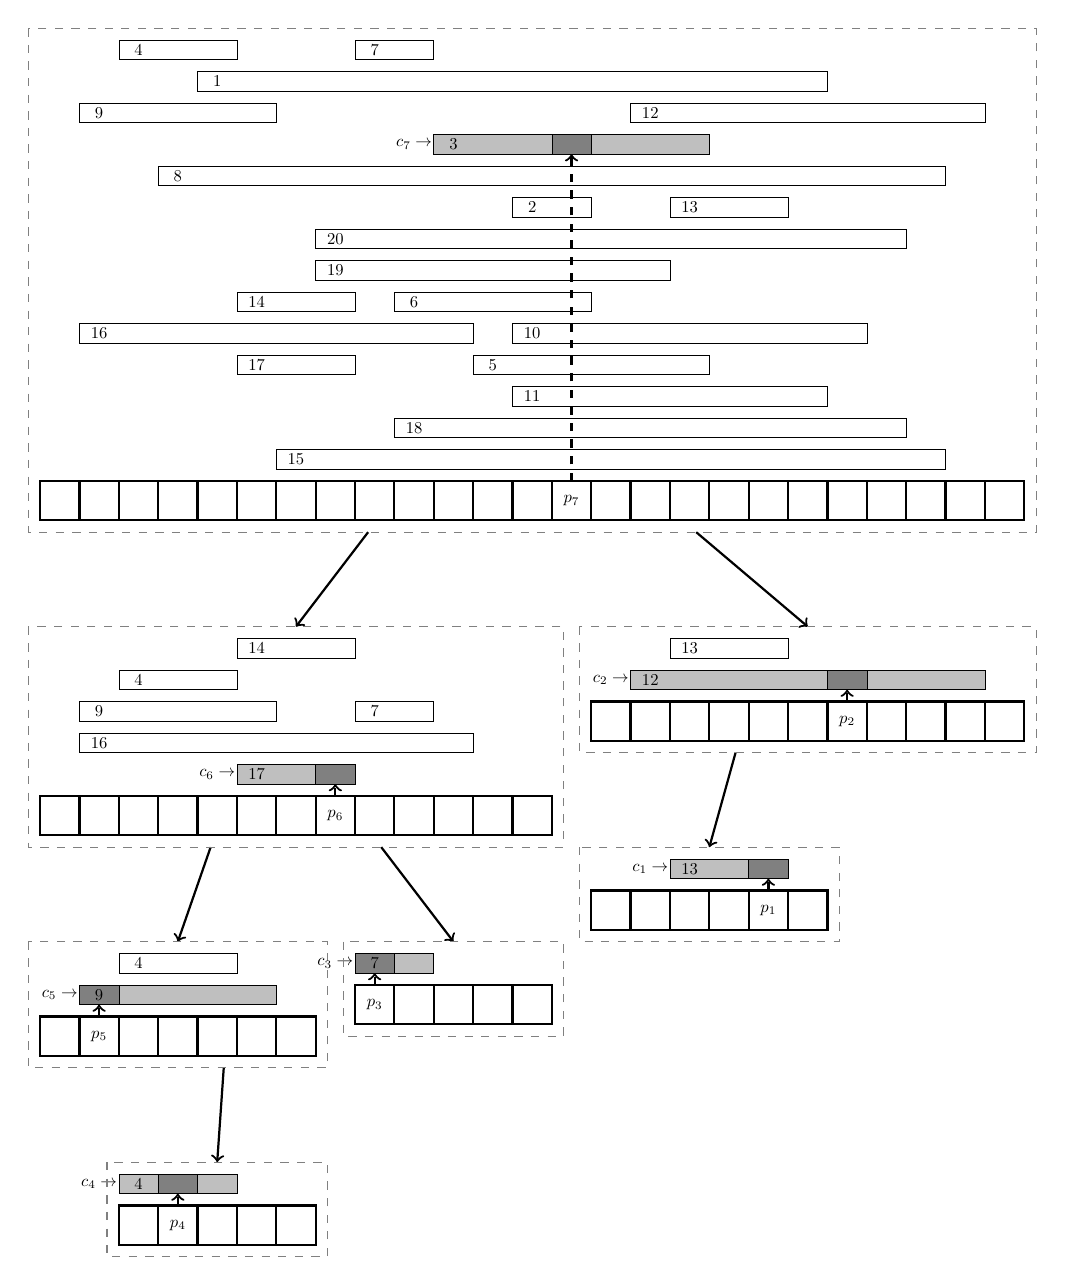
\begin{tikzpicture}[scale=0.5]
\draw[very thin] (2,-3.000000) rectangle (5, -3.500000);
\node[scale=0.6] at (2.500000,-3.250000) {$4$};
\draw[very thin] (8,-3.000000) rectangle (10, -3.500000);
\node[scale=0.6] at (8.500000,-3.250000) {$7$};
\draw[very thin] (4,-3.800000) rectangle (20, -4.300000);
\node[scale=0.6] at (4.500000,-4.050000) {$1$};
\draw[very thin] (1,-4.600000) rectangle (6, -5.100000);
\node[scale=0.6] at (1.500000,-4.850000) {$9$};
\draw[very thin] (15,-4.600000) rectangle (24, -5.100000);
\node[scale=0.6] at (15.500000,-4.850000) {$12$};
\draw[very thin,fill=lightgray] (10,-5.400000) rectangle (17, -5.900000);
\draw[very thin,fill=black!50] (13.000000,-5.400000) rectangle (14.000000,-5.900000);
\node[scale=0.6] at (10.500000,-5.650000) {$3$};
\node[scale=0.6] at (9.500000,-5.650000) {$c_7 \rightarrow$};
\draw[very thin] (3,-6.200000) rectangle (23, -6.700000);
\node[scale=0.6] at (3.500000,-6.450000) {$8$};
\draw[very thin] (16,-7.000000) rectangle (19, -7.500000);
\node[scale=0.6] at (16.500000,-7.250000) {$13$};
\draw[very thin] (12,-7.000000) rectangle (14, -7.500000);
\node[scale=0.6] at (12.500000,-7.250000) {$2$};
\draw[very thin] (7,-7.800000) rectangle (22, -8.300000);
\node[scale=0.6] at (7.500000,-8.050000) {$20$};
\draw[very thin] (7,-8.600000) rectangle (16, -9.100000);
\node[scale=0.6] at (7.500000,-8.850000) {$19$};
\draw[very thin] (5,-9.400000) rectangle (8, -9.900000);
\node[scale=0.6] at (5.500000,-9.650000) {$14$};
\draw[very thin] (9,-9.400000) rectangle (14, -9.900000);
\node[scale=0.6] at (9.500000,-9.650000) {$6$};
\draw[very thin] (1,-10.200000) rectangle (11, -10.700000);
\node[scale=0.6] at (1.500000,-10.450000) {$16$};
\draw[very thin] (12,-10.200000) rectangle (21, -10.700000);
\node[scale=0.6] at (12.500000,-10.450000) {$10$};
\draw[very thin] (11,-11.000000) rectangle (17, -11.500000);
\node[scale=0.6] at (11.500000,-11.250000) {$5$};
\draw[very thin] (5,-11.000000) rectangle (8, -11.500000);
\node[scale=0.6] at (5.500000,-11.250000) {$17$};
\draw[very thin] (12,-11.800000) rectangle (20, -12.300000);
\node[scale=0.6] at (12.500000,-12.050000) {$11$};
\draw[very thin] (9,-12.600000) rectangle (22, -13.100000);
\node[scale=0.6] at (9.500000,-12.850000) {$18$};
\draw[very thin] (6,-13.400000) rectangle (23, -13.900000);
\node[scale=0.6] at (6.500000,-13.650000) {$15$};
\draw[thick] (1.000000,-14.200000) -- (1.000000,-15.200000);
\draw[thick] (2.000000,-14.200000) -- (2.000000,-15.200000);
\draw[thick] (3.000000,-14.200000) -- (3.000000,-15.200000);
\draw[thick] (4.000000,-14.200000) -- (4.000000,-15.200000);
\draw[thick] (5.000000,-14.200000) -- (5.000000,-15.200000);
\draw[thick] (6.000000,-14.200000) -- (6.000000,-15.200000);
\draw[thick] (7.000000,-14.200000) -- (7.000000,-15.200000);
\draw[thick] (8.000000,-14.200000) -- (8.000000,-15.200000);
\draw[thick] (9.000000,-14.200000) -- (9.000000,-15.200000);
\draw[thick] (10.000000,-14.200000) -- (10.000000,-15.200000);
\draw[thick] (11.000000,-14.200000) -- (11.000000,-15.200000);
\draw[thick] (12.000000,-14.200000) -- (12.000000,-15.200000);
\draw[thick] (13.000000,-14.200000) -- (13.000000,-15.200000);
\draw[thick] (14.000000,-14.200000) -- (14.000000,-15.200000);
\draw[thick] (15.000000,-14.200000) -- (15.000000,-15.200000);
\draw[thick] (16.000000,-14.200000) -- (16.000000,-15.200000);
\draw[thick] (17.000000,-14.200000) -- (17.000000,-15.200000);
\draw[thick] (18.000000,-14.200000) -- (18.000000,-15.200000);
\draw[thick] (19.000000,-14.200000) -- (19.000000,-15.200000);
\draw[thick] (20.000000,-14.200000) -- (20.000000,-15.200000);
\draw[thick] (21.000000,-14.200000) -- (21.000000,-15.200000);
\draw[thick] (22.000000,-14.200000) -- (22.000000,-15.200000);
\draw[thick] (23.000000,-14.200000) -- (23.000000,-15.200000);
\draw[thick] (24.000000,-14.200000) -- (24.000000,-15.200000);
\draw[thick] (0.000000,-14.200000) rectangle (25.000000,-15.200000);
\node[scale=0.6] at (13.500000,-14.700000) {$p_7$};
\draw[thick,dashed,->] (13.500000,-14.200000) -- (13.500000,-5.900000);
\draw[thick,->] (8.333333,-15.500000) -- (6.500000,-17.900000);
\draw[very thin] (5,-18.200000) rectangle (8, -18.700000);
\node[scale=0.6] at (5.500000,-18.450000) {$14$};
\draw[very thin] (2,-19.000000) rectangle (5, -19.500000);
\node[scale=0.6] at (2.500000,-19.250000) {$4$};
\draw[very thin] (8,-19.800000) rectangle (10, -20.300000);
\node[scale=0.6] at (8.500000,-20.050000) {$7$};
\draw[very thin] (1,-19.800000) rectangle (6, -20.300000);
\node[scale=0.6] at (1.500000,-20.050000) {$9$};
\draw[very thin] (1,-20.600000) rectangle (11, -21.100000);
\node[scale=0.6] at (1.500000,-20.850000) {$16$};
\draw[very thin,fill=lightgray] (5,-21.400000) rectangle (8, -21.900000);
\draw[very thin,fill=black!50] (7.000000,-21.400000) rectangle (8.000000,-21.900000);
\node[scale=0.6] at (5.500000,-21.650000) {$17$};
\node[scale=0.6] at (4.500000,-21.650000) {$c_6 \rightarrow$};
\draw[thick] (1.000000,-22.200000) -- (1.000000,-23.200000);
\draw[thick] (2.000000,-22.200000) -- (2.000000,-23.200000);
\draw[thick] (3.000000,-22.200000) -- (3.000000,-23.200000);
\draw[thick] (4.000000,-22.200000) -- (4.000000,-23.200000);
\draw[thick] (5.000000,-22.200000) -- (5.000000,-23.200000);
\draw[thick] (6.000000,-22.200000) -- (6.000000,-23.200000);
\draw[thick] (7.000000,-22.200000) -- (7.000000,-23.200000);
\draw[thick] (8.000000,-22.200000) -- (8.000000,-23.200000);
\draw[thick] (9.000000,-22.200000) -- (9.000000,-23.200000);
\draw[thick] (10.000000,-22.200000) -- (10.000000,-23.200000);
\draw[thick] (11.000000,-22.200000) -- (11.000000,-23.200000);
\draw[thick] (12.000000,-22.200000) -- (12.000000,-23.200000);
\draw[thick] (0.000000,-22.200000) rectangle (13.000000,-23.200000);
\node[scale=0.6] at (7.500000,-22.700000) {$p_6$};
\draw[thick,dashed,->] (7.500000,-22.200000) -- (7.500000,-21.900000);
\draw[thick,->] (4.333333,-23.500000) -- (3.500000,-25.900000);
\draw[very thin] (2,-26.200000) rectangle (5, -26.700000);
\node[scale=0.6] at (2.500000,-26.450000) {$4$};
\draw[very thin,fill=lightgray] (1,-27.000000) rectangle (6, -27.500000);
\draw[very thin,fill=black!50] (1.000000,-27.000000) rectangle (2.000000,-27.500000);
\node[scale=0.6] at (1.500000,-27.250000) {$9$};
\node[scale=0.6] at (0.500000,-27.250000) {$c_5 \rightarrow$};
\draw[thick] (1.000000,-27.800000) -- (1.000000,-28.800000);
\draw[thick] (2.000000,-27.800000) -- (2.000000,-28.800000);
\draw[thick] (3.000000,-27.800000) -- (3.000000,-28.800000);
\draw[thick] (4.000000,-27.800000) -- (4.000000,-28.800000);
\draw[thick] (5.000000,-27.800000) -- (5.000000,-28.800000);
\draw[thick] (6.000000,-27.800000) -- (6.000000,-28.800000);
\draw[thick] (0.000000,-27.800000) rectangle (7.000000,-28.800000);
\node[scale=0.6] at (1.500000,-28.300000) {$p_5$};
\draw[thick,dashed,->] (1.500000,-27.800000) -- (1.500000,-27.500000);
\draw[thick,->] (4.666667,-29.100000) -- (4.500000,-31.500000);
\draw[very thin,fill=lightgray] (2,-31.800000) rectangle (5, -32.300000);
\draw[very thin,fill=black!50] (3.000000,-31.800000) rectangle (4.000000,-32.300000);
\node[scale=0.6] at (2.500000,-32.050000) {$4$};
\node[scale=0.6] at (1.500000,-32.050000) {$c_4 \rightarrow$};
\draw[thick] (3.000000,-32.600000) -- (3.000000,-33.600000);
\draw[thick] (4.000000,-32.600000) -- (4.000000,-33.600000);
\draw[thick] (5.000000,-32.600000) -- (5.000000,-33.600000);
\draw[thick] (6.000000,-32.600000) -- (6.000000,-33.600000);
\draw[thick] (2.000000,-32.600000) rectangle (7.000000,-33.600000);
\node[scale=0.6] at (3.500000,-33.100000) {$p_4$};
\draw[thick,dashed,->] (3.500000,-32.600000) -- (3.500000,-32.300000);
\draw[thin,dashed,black!50] (1.700000,-31.500000) rectangle (7.300000,-33.900000);
\draw[thin,dashed,black!50] (-0.300000,-25.900000) rectangle (7.300000,-29.100000);
\draw[thick,->] (8.666667,-23.500000) -- (10.500000,-25.900000);
\draw[very thin,fill=lightgray] (8,-26.200000) rectangle (10, -26.700000);
\draw[very thin,fill=black!50] (8.000000,-26.200000) rectangle (9.000000,-26.700000);
\node[scale=0.6] at (8.500000,-26.450000) {$7$};
\node[scale=0.6] at (7.500000,-26.450000) {$c_3 \rightarrow$};
\draw[thick] (9.000000,-27.000000) -- (9.000000,-28.000000);
\draw[thick] (10.000000,-27.000000) -- (10.000000,-28.000000);
\draw[thick] (11.000000,-27.000000) -- (11.000000,-28.000000);
\draw[thick] (12.000000,-27.000000) -- (12.000000,-28.000000);
\draw[thick] (8.000000,-27.000000) rectangle (13.000000,-28.000000);
\node[scale=0.6] at (8.500000,-27.500000) {$p_3$};
\draw[thick,dashed,->] (8.500000,-27.000000) -- (8.500000,-26.700000);
\draw[thin,dashed,black!50] (7.700000,-25.900000) rectangle (13.300000,-28.300000);
\draw[thin,dashed,black!50] (-0.300000,-17.900000) rectangle (13.300000,-23.500000);
\draw[thick,->] (16.666667,-15.500000) -- (19.500000,-17.900000);
\draw[very thin] (16,-18.200000) rectangle (19, -18.700000);
\node[scale=0.6] at (16.500000,-18.450000) {$13$};
\draw[very thin,fill=lightgray] (15,-19.000000) rectangle (24, -19.500000);
\draw[very thin,fill=black!50] (20.000000,-19.000000) rectangle (21.000000,-19.500000);
\node[scale=0.6] at (15.500000,-19.250000) {$12$};
\node[scale=0.6] at (14.500000,-19.250000) {$c_2 \rightarrow$};
\draw[thick] (15.000000,-19.800000) -- (15.000000,-20.800000);
\draw[thick] (16.000000,-19.800000) -- (16.000000,-20.800000);
\draw[thick] (17.000000,-19.800000) -- (17.000000,-20.800000);
\draw[thick] (18.000000,-19.800000) -- (18.000000,-20.800000);
\draw[thick] (19.000000,-19.800000) -- (19.000000,-20.800000);
\draw[thick] (20.000000,-19.800000) -- (20.000000,-20.800000);
\draw[thick] (21.000000,-19.800000) -- (21.000000,-20.800000);
\draw[thick] (22.000000,-19.800000) -- (22.000000,-20.800000);
\draw[thick] (23.000000,-19.800000) -- (23.000000,-20.800000);
\draw[thick] (24.000000,-19.800000) -- (24.000000,-20.800000);
\draw[thick] (14.000000,-19.800000) rectangle (25.000000,-20.800000);
\node[scale=0.6] at (20.500000,-20.300000) {$p_2$};
\draw[thick,dashed,->] (20.500000,-19.800000) -- (20.500000,-19.500000);
\draw[thick,->] (17.666667,-21.100000) -- (17.000000,-23.500000);
\draw[very thin,fill=lightgray] (16,-23.800000) rectangle (19, -24.300000);
\draw[very thin,fill=black!50] (18.000000,-23.800000) rectangle (19.000000,-24.300000);
\node[scale=0.6] at (16.500000,-24.050000) {$13$};
\node[scale=0.6] at (15.500000,-24.050000) {$c_1 \rightarrow$};
\draw[thick] (15.000000,-24.600000) -- (15.000000,-25.600000);
\draw[thick] (16.000000,-24.600000) -- (16.000000,-25.600000);
\draw[thick] (17.000000,-24.600000) -- (17.000000,-25.600000);
\draw[thick] (18.000000,-24.600000) -- (18.000000,-25.600000);
\draw[thick] (19.000000,-24.600000) -- (19.000000,-25.600000);
\draw[thick] (14.000000,-24.600000) rectangle (20.000000,-25.600000);
\node[scale=0.6] at (18.500000,-25.100000) {$p_1$};
\draw[thick,dashed,->] (18.500000,-24.600000) -- (18.500000,-24.300000);
\draw[thin,dashed,black!50] (13.700000,-23.500000) rectangle (20.300000,-25.900000);
\draw[thin,dashed,black!50] (13.700000,-17.900000) rectangle (25.300000,-21.100000);
\draw[thin,dashed,black!50] (-0.300000,-2.700000) rectangle (25.300000,-15.500000);
\end{tikzpicture}

    \caption{রেঞ্জগুলো রিকার্সিভলি নির্বাচন করার একটি উপায়।}
    \label{greedy_pie_eaters:1}
  \end{figure}
  এরপর মনে করো $[1, p_K)$-তে রেঞ্জ নির্বাচন করবো। খেয়াল করো, এখন কিন্তু যেই
  গরুগুলো নির্বাচন করবো সেগুলো কিন্তু সম্পুর্নভাবে $[1, p_K)$ রেঞ্জের ভিতর
  থাকতে হবে। এবার মনে করো $d_{K-1}$ এবং $p_{K-1}$ নির্বাচন করলা $[1, p_K)$
  রেঞ্জ থেকে। এর জন্য যেই ২টি সাব-প্রবলেম পাবো আমরা তা হলো $[1, p_{K-1})$ এবং
  $(p_{k-1}, p_{K}]$। এভাবে যেতে থাকলে বুঝতে পারবা আমাদের ডিপি স্টেট বা
  সাব-প্রবলেমকে আমরা ২টি ভ্যালূ দিয়ে প্রকাশ করতে পারি-- $l$ এবং $r$, এবং
  $\DP\two{l}{r}$ দিয়ে বুঝানো হবে $l \ldots r$ এই পাই গুলো এবং পুরাপুরি $[l,
  r]$ এর ভিতরে থাকা গরুগুলোকে বিবেচনা করে একটি $c$ সিকুয়েন্স বাছাই করার
  ম্যাক্সিমাম প্রফিট কতো হতে পারে। আর ডিপি রিকারেন্স হবেঃ
  \[
    \DP\two{l}{r} = \max_{c,\, l \le l_c \le r_c \le r} \max_{p \in [l_c,
    r_c]} \DP\two{l}{p-1} + \DP\two{p+1}{r} + w_c
  \]
  এর রিকারেন্সের কমপ্লেক্সিটি হলো $O(n^3m)$। অবশ্য এটাকে একটু অন্যভাবে দেখলে
  খেয়াল করবা আমাদের আগে গরু ঠিক করে তারপর তার জন্য বরাদ্দ করার জন্য ইনডেক্স
  ঠিক না করে বরং আগে বরাদ্দকৃত ইনডেক্স ফিক্স করে তারপর ওই ইনডেক্সের উপরে দিয়ে
  যায় এমন রেঞ্জগুলোর মধ্যে ম্যাক্সিমাম $w$ যার, তাকে নির্বাচন করলেই হয়।
  সুতরাং আমাদের নতুন রিকারেন্স হবেঃ
  \[
    \DP\two{l}{r} = \max_{p \in [l, r]} \DP\two{l}{p-1} + \DP\two{p+1}{r} +
    f\three{l}{r}{p}
  \]
  যেখানে $f\three{l}{r}{p}$ হলো যেসব রেঞ্জ পুরাপুরি $[l, r]$ রেঞ্জের ভিতরে
  আছে এবং $p$ এর উপরে দিয়ে যায়, তাদের মধ্যে ম্যাক্সিমাম $w$ এর মান। শুরুতে
  আমাদের $f$ টেবিলটা প্রি-ক্যাল্কুলেট করে নিতে হবে $O(n^3)$ টাইমের মধ্যে।
  এটাও একটা ছোটোখাটো ডিপি প্রবলেম বলতে পারো, রিকারেন্স এর সাহায্যে
  ক্যাল্কুলেট করে নিতে পারবা। পাঠকের অনুশীলনের জন্য রেখে দেওয়া হলো।
\end{solution}

\begin{example}[\href{https://codeforces.com/contest/1146/problem/%
  G}{Codeforces 1146G - Zoning Restrictions}]
  তুমি $n$ টা বিল্ডিং বানাবে, এবং বিল্ডিং বানানোর স্পটগুলো $1$ থেকে $n$
  পর্যন্ত নাম্বারিং করা। প্রতিটা বিল্ডিঙের উচ্চতা 0 থেকে $h$ এর মধ্যে যেকোনো
  একটি পর্ণসংখ্যা হতে পারে। কোন স্পটে যদি $a$ উচ্চতার বিল্ডিং বানাও তাহলে
  তুমি $a^2$ টাকা পাবা। তুমি যাতে ইচ্ছা মতো উচ্চতার বিল্ডিং নির্মাণ করতে না
  পারো তাই $m$ টা শর্ত দেওয়া আছে -- $i$ তম শর্তে তোমাকে বলা আছে $l_i$ থেকে
  $r_i$ স্পটের বিল্ডিং গুলোর উচ্চতা সর্বোচ্চ $v_i$ হতে পারবে। যদি এদের মধ্যে
  কোনটার উচ্চতা $v_i$ এর বেশি হয় তাহলে তোমাকে $c_i$ টাকা পেনাল্টি দিতে হবে।
  খেয়াল করো, $l_i$ থেকে $r_i$ এর মধ্যে একাধিক বিল্ডিং-এর উচ্চতা $v_i$ এর
  চাইতে বেশি হলেও কিন্তু $i$-তম শর্ত ভঙ্গের জন্য একবারই $c_i$ টাকা পেনাল্টি
  দিবে। অপ্টিমালভাবে বিল্ডিং-এর উচ্চতা নির্বাচন করে ম্যাক্সিমাম কতো প্রফিট
  পেতে পারো তা হিসাব করো। $1 \le n, m, h \le 50, 1 \le l_i \le r_i \le n, 0
  \le v_i \le h, 1 \le c_i \le 5\,000$।
\end{example}
\begin{solution}
  এই প্রব্লেমটা কিছুটা আগের প্রব্লেমের মতো। ধরো তুমি প্রথমে একটা বিল্ডিং $i$
  নির্মাণ করবা ঠিক করেছো। এই $i$ নাম্বার বিনল্ডিংটি কিছু কিছু শর্ত ভাঙ্গবে,
  সেগুলোর পেনাল্টি ধরো তুমি দিয়ে দিলে। এখন পরের বিল্ডিংগুলো যখন নির্মাণ করতে
  যাবে, তখন $i$ বিল্ডিঙের জন্য কোন কোন শর্ত ভাঙ্গা হয়েছিলো আর কোনগুলোর
  পেনাল্টি তুমি হিসাবে নিয়ে ফেলেছ এগুলো ট্র্যাক রাখা একটু জটিল হয়ে যাবে। এর
  জন্য আমরা যেটা করবো তা হলো, প্রথম বিল্ডিংটি এমনভাবে নির্মাণ করবো যেন
  সেটা সব বিল্ডিংগুলোর মধ্যে ম্যাক্সিমাম উচ্চতার বিল্ডিংগুলোর একটি হয়। এটা
  করে কি লাভ আমাদের? এটা করার ফলে, এই বিল্ডিংটি নির্মাণ করতে গিয়ে যেইসব
  শর্তের রেঞ্জ গুলো $i$ নাম্বার বিল্ডিংটির উপর দিয়ে গিয়েছে তাদের মধ্যে যেগুলো
  মানা হয়নি তাদের পেনাল্টি আমরা এখনি হিসাবে নিয়ে নিবো, আর যেগুলো ভাঙ্গা হয়নি
  সেগুলো সামনেও কখনো ভাঙ্গা হবে না কারণ ভবিষ্যতের বিল্ডিংগুলোর উচ্চতা
  সর্বোচ্চ $i$ নাম্বার বিল্ডিঙের উচ্চতার সমান হবে। সেগুলো পরের অন্য বিল্ডিং
  গুলো নির্মাণের সময় বিবেচনায় রাখারই দরকার নেই। মোটকথা, $i$ নাম্বার
  বিল্ডিং-এর উপর দিয়ে যেই রেঞ্জ গুলো গিয়েছে তাদের আমরা বিবেচনা করে ফেলেছি, আর
  ভবিষ্যতে তাদের বিবেচনা করতে হবে না। বাকি যেই রেঞ্জ গুলো আছে, সেগুলো আগের
  প্রব্লেমের মতই হয় পুরোপুরি $i$ এর বামে হবে, নাহয় পুরোপুরি ডানে হবে, এবং
  একইভাবে ২টা ইন্ডিপেন্ডেন্ট সাব-প্রবলেম পাবো।
  
  এখন কথা হচ্ছে আমরা $i$ নাম্বার বিল্ডিংটি যাতে সর্বোচ্চ বিল্ডিং গুলোর একটি
  হয় সেটা নিশ্চিত করবো কিভাবে? এটার জন্য আমরা ডিপিতে আরেকটি স্টেট রাখবোঃ
  নির্মানকৃত বিল্ডিং গুলোর উচ্চতা সর্বোচ্চ কত হতে পারবে, তাহলে আমরা অনেকটা
  এরকম ইনফরমেশন পাস করতে পারবোঃ ``এই ২টি সাব-প্রবলেমের মধ্যে বিল্ডিং এর
  সর্বোচ্চ উচ্চতা $i$ তম বিল্ডিং এর সমান হতে পারবে''।

  সুতরাং আমাদের ডিপির স্টেট ৩টা হবেঃ $l$, $r$ এবং $x$, আর
  $\DP\three{l}{r}{x}$ এর মানে হলো শুধুমাত্র সেইসব শর্তগুলো, যেগুলোর রেঞ্জ
  সম্পূর্ণ $[l, r]$ এর ভিতরে, সেগুলো বিবেচনা করে $l \ldots r$ বিল্ডিংগুলো
  নির্মাণ করে ম্যাক্সিমাম কত প্রফিট পাওয়া যায় যাতে কোন বিল্ডিং-এর উচ্চতা $x$
  এর বেশি না হয়। $\DP\three{l}{r}{x}$ ক্যাল্কুলেট করার জন্য আমরা সর্বোচ্চ
  বিল্ডিং কোনটা সেটার উপরে, এবং সেই বিল্ডিং-এর উচ্চতা কতোটুক হবে -- এই ২টির
  উপর ইটারেট করবো। তাহলে রিকারেন্সটা হবেঃ
  \[
    \DP\three{l}{r}{x} = \max_{l \le i \le r, 0 \le y \le x}
    \DP\three{l}{i-1}{y} + \DP\three{i+1}{r}{y} - f\four{l}{r}{i}{y} + y^2
  \], যেখানে $f\four{l}{r}{i}{y}$ হলো এমন সব শর্ত $j$, যেগুলো সম্পূর্ণভাবে
  $[l, r]$ এর ভিতরে, $i$ এর উপর দিয়ে গিয়েছে, এবং $v_j < y$, তাদের $c_j$ এর
  যোগফল।
\end{solution}

% \begin{example}[\href{http://www.usaco.org/index.php?page=viewproblem2%
%   &cpid=698}{USACO - Subsequence Reversal}]
%   তোমাকে একটা অ্যারে $a_1, a_2, \ldots, a_N$ দেওয়া আছে। প্রথমে এই অ্যারের
%   একটি সাবসিকুয়েন্স নির্বাচন করে তা রিভার্স করবা, এবং এরপর যেই অ্যারেটা পাবা
%   তার Longest Non-decreasing সাবসিকুয়েন্স বের করবা। তোমার উদ্দেশ্য হচ্ছে, যেই
%   সাবসিকুয়েন্সটা রিভার্স করবা, সেটা এমনভাবে নির্বাচন করা, যাতে Longest
%   Non-decreasing সাবসিকুয়েন্স সর্বোচ্চ হয়। যেমন, নিচের অ্যারেটির গাড় করা
%   সাবসিকুয়েন্স নির্বাচন করে সেটি রিভার্স করলে পুরো অ্যারেটিই Non-decreasing
%   হয়ে যায়। $1 \le N, a_i \le 50$।
%   \begin{center}
%     \begin{tabular}{|c|c|c|c|c|c|c|c|c|}
%       \hline
%       1 & 2 & 3 & \cellcolor{black!25}9 & 5 & 6 & \cellcolor{black!25}8 &
%       \cellcolor{black!25}7 & \cellcolor{black!25}4 \\
%       \hline
%     \end{tabular}\\
%     $\downarrow$\\
%     \begin{tabular}{|c|c|c|c|c|c|c|c|c|}
%       \hline
%       1 & 2 & 3 & \cellcolor{black!25}4 & 5 & 6 & \cellcolor{black!25}7 &
%       \cellcolor{black!25}8 & \cellcolor{black!25}9 \\
%       \hline
%     \end{tabular}
%   \end{center}
% \end{example}

\begin{example}[\href{https://codeforces.com/contest/1107/problem/E}%
  {Codeforces 1107E - Vasya and Binary String}]
  তোমার কাছে $n$ লেংথের একটি বাইনারি স্ট্রিং $s$, এবং $n$ সাইজের একটি অ্যারে
  $s$ আছে। স্ট্রিংটা খালি না হয়ে যাওয়া পর্যন্ত তুমি এই অপারেশনটি অ্যাপ্লাই
  করবাঃ $s$ এর মধ্যে একটা কন্সেকিউটিভ সাবস্ট্রিং বাছাই করবা যাতে সেই
  সাবস্ট্রিং এর সব ক্যারেক্টার একই হয়, এবং সেই সাবস্ট্রিংটা ডিলিট করে এরপর ২
  পাশের বাকি থাকা সাবস্ট্রিংগুলো (এগুলোর কোনটা ফাকা হলে সমস্যা নেই) জোড়া
  লাগিয়ে দিবা। যেমন 1\colorbox{black!25}{111}101 $\rightarrow$ 1101। $x$
  লেংথের সাবস্ট্রিং ডিলিট করলে $a_x$ পয়েন্ট পাবে। ম্যাক্সিমাম কতো পয়েন্ট
  পেতে পারো তুমি? $1 \le n \le 100, 1 \le a_i \le 10^9$।
\end{example}
\begin{solution}
  এখানেও আমরা উল্টা দিক থেকে চিন্তা করবো। একদম শেষ অপারেশনটার কথা চিন্তা করো
  -- সেখানে সবগুলো ক্যারেক্টার একই হবে। কিন্তু সেগুলা একসাথে জড়ো হওয়ার আছে
  নিশ্চয়ই প্রাথমিক অ্যারেতে কোনো সাব-সিকুয়েন্স হিসেবে ছিল!
  \begin{figure}[h]
    \centering
    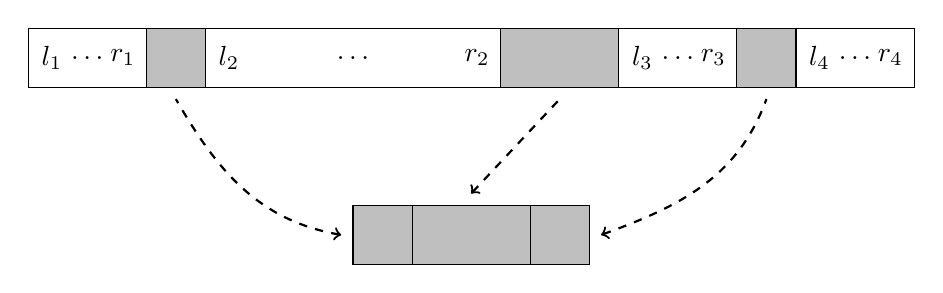
\begin{tikzpicture}[scale=0.75]
      \draw[draw=none,fill=lightgray] (2, 4) rectangle (3, 5);
      \draw[draw=none,fill=lightgray] (8, 4) rectangle (10, 5);
      \draw[draw=none,fill=lightgray] (12, 4) rectangle (13, 5);
      \draw[draw=none,fill=lightgray] (5.5, 1) rectangle (9.5, 2);
      \draw (5.5, 1) rectangle (9.5, 2);
      \draw (6.5, 1) -- (6.5, 2);
      % \draw (7.5, 1) -- (7.5, 2);
      \draw (8.5, 1) -- (8.5, 2);
      \draw (0, 4) rectangle (15, 5);
      \draw (2, 4) -- (2, 5);
      \draw (3, 4) -- (3, 5);
      \draw (8, 4) -- (8, 5);
      \draw (10, 4) -- (10, 5);
      \draw (12, 4) -- (12, 5);
      \draw (13, 4) -- (13, 5);
      \node at (0.4, 4.5) {$l_1$};
      \node at (1.6, 4.5) {$r_1$};
      \node at (3.4, 4.5) {$l_2$};
      \node at (10.4, 4.5) {$l_3$};
      \node at (13.4, 4.5) {$l_4$};
      \node at (7.6, 4.5) {$r_2$};
      \node at (11.6, 4.5) {$r_3$};
      \node at (14.6, 4.5) {$r_4$};
      \node at (1, 4.5) {$\dots$};
      \node at (5.5, 4.5) {$\dots$};
      \node at (11, 4.5) {$\dots$};
      \node at (14, 4.5) {$\dots$};
      \draw[<-, thick, dashed] (5.3, 1.5) to [out=170,in=-60] (2.5, 3.8);
      \draw[<-, thick, dashed] (7.5, 2.2) -- (9, 3.8);
      \draw[<-, thick, dashed] (9.7, 1.5) to [out=20,in=-110] (12.5, 3.8);
    \end{tikzpicture}
  \end{figure}
  চিত্রে এমন একটা উদাহরণ দেখানো হয়েছে। নিচের অ্যারেটি পেতে হলে আগে তোমাকে
  $l_1 \ldots r_1$, $l_2 \ldots r_2$, $l_3 \ldots r_3$ এবং $l_4 \ldots r_4$
  রেঞ্জগুলো ডিলিট করতে হবে। আর এই রেঞ্জগুলো একেকটা সাব-প্রবলেম, যারা
  পুরোপুরি ইন্ডিপেন্ডেন্ট!

  তাহলে বুঝতে পারছো আমাদের ডিপিতে যেই ২টা স্টেট থাকতেই হবে সেগুলো হলো $l$ এবং
  $r$ -- অ্যারের একটি রেঞ্জ। এরপর ট্রানজিশন করার সময় আমরা এই রেঞ্জের একটা সাব
  -সিকুয়েন্স বাছাই করতে পারি যার সব ক্যারেক্টার একই। ধরো সাব-সিকুয়েন্সটির
  লেংথ $x$, তাহলে আমরা $a_x$ অ্যাড করবো, আর সাব-সিকুয়েন্স-এর মাঝে মাঝে যেই
  সাব-অ্যারে গুলো পাবো সেগুলোর ডিপি ভ্যালু গুলো যোগ করবো। কিন্তু এভাবে করলে
  আমাদের ট্রানজিশন এক্সপোনেনশিয়াল সংখ্যক হয়ে যাচ্ছে।

  এর জন্য আমরা যেটা করবো সেটা হলো বাম থেকে ডানে সাব-সিকুয়েন্স একটা একটা
  ইনডেক্স করে বানাবো। খেয়াল করো, সাব-সিকুয়েন্সে কোন কোন ইনডেক্স আছে তা কিন্তু
  আমাদের ট্র্যাক রাখতে হচ্ছে না। আমরা শুধু ট্র্যাক রাখবো ইতোমধ্যে কয়টা
  ইনডেক্স নিয়ে ফেলেছি সাব-সিকুয়েন্সে।

  এই সবগুলো আইডিয়া মিলিয়ে আমরা যেই ডিপি পাচ্ছি তা হলো, $\DP\three{l}{r}{x}$,
  যার মানে হলো আমাদেরকে $s[l \ldots r]$ পুরোটা ডিলিট করতে হবে, সাথে বলা আছেঃ
  $s[1 \ldots (l-1)]$ এর কিছু কিছু সাব-অ্যারে ডিলিট করে আমাদের কাছে $s[1
  \ldots (l-1)]$ এর যেই সাব-সিকুয়েন্স বাকি আছে, তার লেংথ $x$ এবং এদের সবার
  ক্যারেক্টার $s_l$ এর সমান।

  ট্রানজিশন গুলো হবেঃ
  \begin{enumerate}
    \item আমরা শুরুতে যেই সাব-সিকুয়েন্স বাছাই করা শুরু করেছিলাম, সেটার শেষ
    ইন্ডেক্সটাই হলো $l$, তাহলে আগের $x$ টা ইনডেক্সসহ মিলে মোট $x+1$ লেংথ এর
    একটা সাব-সিকুয়েন্স পাচ্ছি, এর পয়েন্ট হলো $a_{x+1}$। এরপর আবার আমাদেরকে
    $s[l+1 \ldots r]$ এই সাব অ্যারেটি ডিলিট করতে হবে, সেটার ম্যাক্সিমাম
    পয়েন্ট হলো $\DP\three{l+1}{r}{0}$।
    \item আমরা জানি $s_l$ হলো সাব-সিকুয়েন্সে বাছাই করা উপাদান গুলোর মধ্যে
    একটি। এখন আমরা $(l+1) \ldots r$ রেঞ্জে ইটারেট করবো কোন ইন্ডেক্সটা সেই
    সাব-সিকুয়েন্সের পরবর্তী ইনডেক্স হবে। ধরো সেটা হলো $i$ (এখানে $s_i = s_l$
    হতে হবে কিন্তু!)। তাহলে আমাদের আগে $s[(l+1) \ldots (i-1)]$ কে ডিলিট করতে
    হবে। যার ম্যাক্সিমাম পয়েন্ট হলো $\DP\three{l+1}{i-1}{0}$। এরপর আমাদের
    আগের মতো সাব-সিকুয়েন্স বাছাই করে করে আগাতে হবে, যার ম্যাক্সিমাম পয়েন্ট
    হলো $\DP\three{i}{r}{x+1}$।
  \end{enumerate}

  টাইম কমপ্লেক্সিটি হলো $O(n^3)$।
\end{solution}

\begin{example}[\href{https://codeforces.com/gym/102979/problem/G}%
  {XXI Open Cup, GP of Suwon - Generate The Array}]
  ধরো তোমাকে একটা $N$ লেংথের অ্যারে $A$ দেওয়া আছে, এবং তুমি এতে কিছু কুয়েরি
  করবাঃ অ্যারের একটা সেগমেন্ট $[i, j]$ এর জন্য সেই সেগমেন্টের ম্যাক্সিমাম বের
  করবা, ধরো $[i, j]$ সেগমেন্টের ম্যাক্সিমাম $R_{i,j}$। $[i, j]$ সেগমেন্টটি
  $Q_{i, j}$ বার করা হবে।\\
  কিন্তু অ্যারেটা তোমাকে দেওয়া নাই, তুমি বানাবে সেটা। $1$ থেকে $N$ এর মধ্যে
  প্রতিটা $i$ এর জন্য $A_i$ এর মান হিসেবে তুমি $K_i$ টা আলাদা আলাদা মান
  $V_{i,1}, V_{i,2}, \ldots, V_{i, K_i}$ থেকে একটি বাছাই করতে পারবা। $A_i$ এর
  জন্য $V_{i, j}$ বাছাই করার কস্ট হলো $C_{i, j}$। ধরো, $i$-তম ইনডেক্সের জন্য
  $P_i$-তম ভ্যালুটি বাছাই করেছ, অর্থাৎ $A_i = V_{i,P_i}$।\\
  সবগুলো কুয়েরির শেষে তোমার স্কোর হবেঃ (সব ইন্টারভাল কুয়েরির রেজাল্টের যোগফল)
  $-$ ($A_i$ ভ্যালু গুলা বাছাই করার কস্টের যোগফল)। অর্থাৎ,
  \[
    \text{স্কোর} = \sum_{1 \le i \le j \le N} Q_{i,j} \cdot R_{i,j} - \sum_{i
    = 1}^{N} C_{i,P_i}
  \]। ম্যাক্সিমাম কতো স্কোর পেতে পারো তা বের করো। তোমাকে $N, Q, C, V, K$ দিয়ে
  দেওয়া হবে। $1 \le N \le 300$, $0 \le Q_{i,j} \le 999$, $0 \leq V_{i, j}
  \leq 10^8$, $0 \leq C_{i, j} \leq 10^{13}$, $\sum K_i \le 3\cdot 10^5$।
\end{example}
\begin{solution}
  আগের প্রবলেম গুলোর সলিউশনের আলোচনা থেকে আশা করি বুঝতে পারছো আমাদের এখানে
  একটা রেঞ্জের উপর সাব-প্রবলেম সল্ভ করতে হবে। যেহেতু আমাদেরকে রেঞ্জের
  ম্যাক্সিমাম নিয়ে কাজ করতে হচ্ছে, সেজন্য আমরা আমাদের
  বর্তমান সাব-প্রবলেমের রেঞ্জে (ধরো, $l \ldots r$) কোন ইন্ডেক্সটা ম্যাক্সিমাম
  ভ্যালু হবে তা ঠিক করবো। ধরো $i \in [l, r]$ ইনডেক্সটি হলো ম্যাক্সিমাম
  ভ্যালুর ইনডেক্স। এখন আমরা $i$-তম ইনডেক্সে কোন ভ্যালূ বসাবো তা ঠিক করবো এবং
  $[l, i)$ আর $(i, r]$ ইন্টারভালে রিকার্স করবো -- সাথে বলে দিবো এই ২টি
  ইন্টারভালের ভ্যালূ গুলো $i$-তম ইনডেক্সের ভ্যালুর চেয়ে ছোট হবে।

  সবকিছু গুছালে আমাদের নাইভ সলিউশনটি এমন দাঁড়াবেঃ ডিপির স্টেট ৩টি -- $l$, $r$
  এবং $x$, আর $\DP\three{l}{r}{x}$ এর মানে হলো, $A[l \ldots r]$ এই অ্যারেটা
  বানানো ম্যাক্সিমাম স্কোর, যাতে সব $i \in [l, r]$ এর জন্য $A_i \le x$ হয়। এর
  রিকারেন্স হবেঃ
  \[
    \DP\three{l}{r}{x} = \max_{i=l}^{r} \max_{j=1}^{K_i}
    \DP\three{l}{i-1}{V_{i, j}} + \DP\three{i+1}{r}{V_{i, j}} +
    T\three{l}{r}{i} \cdot V_{i,j} - C_{i,j}
  \], যেখানে $T\three{l}{r}{i}$ হলো $[l, r]$ রেঞ্জের ভিতর আছে এবং $i$ এর উপর
  দিয়ে যায়, এমন কয়টি কুয়েরি আছে, অর্থাৎ $T\three{l}{r}{i} = \sum_{l \le
  l^\prime \le i \le r^\prime \le r} Q_{i,j}$। এটা $O(N^3)$ টাইমের মধ্যে
  প্রি-ক্যাল্কুলেট করে নেওয়া যাবে। এই ডিপির স্টেট আছে $N \times N \times
  \left(\sum_{i=1}^{N} K_i\right)$ টি, আর প্রতি স্টেটে মোটামুটি $O(N) \times
  O(K_i)$ সাইজের লুপ চলছে। আর যাই হোক, আমাদেরকে যেই কন্সট্রেইন্ট গুলো দেওয়া
  হয়েছে, তাতে এই ডিপি কাজ করবে না।

  এখন আমাদের নতুন কিছু অবজারভেশন লাগবে ডিপিটিকে অপ্টিমাইজ করতে।

  \textbf{অপটিমাইজেশন ১ঃ} $l \ldots r$ এর মধ্যে $i$ কে ম্যাক্সিমাম ধরার পর $l
  \ldots (i-1)$ এবং $(i+1) \ldots r$ এর ভ্যালু গুলো যাতে সর্বোচ্চ $i$ এর সমান
  হয়, এটা নিশ্চিত করার দরকার নেই -- ওই ভ্যালূ গুলো যদি $i$ এর চাইতে বড়-ও হয়ে
  যায়, তাহলে সেটা কখনো অপ্টিমাল হবে না, এবং আমাদের ফাইনাল অ্যান্সারে প্রভাব
  ফেলবে না। এর ফলে আমাদের যা লাভ হবে তা হলো আমরা ডিপির তৃতীয় স্টেটটা ($x$)
  বাদ দিয়ে দিতে পারি।

  এই অবজারভেশনটা বুঝার জন্য এভাবে চিন্তা করোঃ ধরো তোমার কাছে $A$ এর ভ্যালু
  গুলা ফিক্স করা আছে। তাহলে একটা জিনিশ খেয়াল করো, এর ফলে কিন্তু আমাদের স্কোর
  ফাংশনের $- \sum_{i = 1}^{N} C_{i,P_i}$ এই অংশটাও ফিক্স হয়ে গিয়েছে।
  \begin{align*}
    \text{স্কোর} = \sum_{1 \le i \le j \le N} Q_{i,j} \cdot R_{i,j}
    \Aboxed{ - \sum_{i = 1}^{N} C_{i,P_i}}
  \end{align*}
  আর বাকি থাকছে শুধু $\sum_{1 \le i \le j \le N} Q_{i,j} \cdot R_{i,j}$
  অংশটা। আমাদের টার্গেট হলো এটাকে ম্যাক্সিমাইজ করা। চিন্তা করে দেখো, আমরা যদি
  ডিপির স্টেটে $x$ কে না রেখে অ্যারের বিভিন্ন সাব-অ্যারের ম্যাক্সিমামকে
  ভুলভাবে চিহ্নিত করি, তাহলে কিন্তু সেটা থেকে যেই $\sum_{1 \le i \le j \le N}
  Q_{i,j} \cdot R_{i,j}$ এর মান পাবো, সেটা সবসময়ই অ্যারের  ম্যাক্সিমাম গুলোকে
  ঠিক মতো আন্দাজ করতে পারলে যেই মান পাবো তার চেয়ে ছোট অথবা সমান হবে। আর
  আমাদের ডিপিতে আমরা যেহেতু ডিপিতে সব উপায়ে আন্দাজ করে করে দেখছি, সেহেতু একটা
  না একটাতে আমরা সঠিকভাবে আন্দাজ করে ফেলবো, এবং আমাদের ফাইনাল অ্যান্সার সবসময়
  ঠিক হবে। তাহলে আমাদের নতুন ডিপিটা হবেঃ
  \[
    \DP\two{l}{r} = \max_{i=l}^{r} \max_{j=1}^{K_i}
    \DP\two{l}{i-1} + \DP\two{i+1}{r} +
    T\three{l}{r}{i} \cdot V_{i,j} - C_{i,j}
  \]

  \textbf{অপটিমাইজেশন ২ঃ} কনভেক্স হাল ট্রিক।

  আগের ডিপি ফরমুলাটাকে আমরা একটু অন্যভাবে লিখতে পারিঃ
  \begin{align*}
    \DP\two{l}{r} = \max_{i=l}^{r}
    \DP\two{l}{i-1} + \DP\two{i+1}{r} +
    \Aboxed{\max_{j=1}^{K_i} T\three{l}{r}{i} \cdot V_{i,j} - C_{i,j}}
  \end{align*}
  আমরা প্রতি $(l, r, i)$ টুপলের জন্য $\max_{j=1}^{K_i} T\three{l}{r}{i} \cdot
  V_{i,j} - C_{i,j}$ এর মান আগে থেকে $O(N^3 + \sum K_i)$ টাইমে বের করে ফেলতে
  পারবো। কিভাবে? যদি তুমি $i$ ফিক্স করো, তাহলে $K_i$ টা $mx + b$ আকারের লাইন
  ইকুয়েশন পাবা, যেখানে $m = V_{i, j}$ এবং $b = - C_{i,j}$। এবার প্রতি $(l,
  r)$ পেয়ারের উপর ইটারেট করে $x = T\three{l}{r}{i}$-তে মিনিমাম ভ্যালু কতো তা
  বের করতে হবে, আর এই প্রবলেমটাই কনভেক্স হাল ট্রিক দিয়ে সল্ভ করা হয়।
  বিস্তারিত পড়তে চাইলে কনভেক্স হাল ট্রিক চ্যাপ্টারটি পড়ো।

  % আমরা ডিপিটাকে অপ্টিমাইজ করবো। প্রথম অপটিমাইজেশন একটু ট্রিকি কিন্তু খুবই
  % সুন্দর! খেয়াল করে দেখো, আমরা কিন্তু ডিপির তৃতীয় ডাইমেনশনটাকে বাদ দিয়ে দিতে
  % পারি! কিন্তু, আমরা যদি ট্র্যাক না রাখি এখন পর্যন্ত ম্যাক্সিমাম ভ্যালূ
  % যেগুলো নির্বাচন করে এসেছি তাদের মধ্যে মিনিমাম কোনটা, তাহলে বর্তমান ইনডেক্সে
  % যখন একটা ভ্যালূ ঠিক করতে যাবো তখন তো সেটা আগের ম্যাক্সিমাম ভ্যালূর চাইতে
  % বেশি হয়ে যেতে পারে; এটা তো আমাদের প্রাথমিক ট্রিকটাই নষ্ট করে দিবে, কারণ
  % আমরা ধরেই নিয়েছিলাম, আমরা যেই ভ্যালু অ্যাাসাইন করে আসছি সেগুলো নির্দিষ্ট
  % কিছু রেঞ্জের মধ্যে ম্যাক্সিমাম, আর তাদের কাছ থেকেই আমরা কুয়েরির
  % কন্ট্রিবিউশন গুলো পাচ্ছি। আরেক্টু ভালোভাবে চিন্তা করে দেখা যাক বিষয়টাকে।
  % ধরো, $l \ldots r$ এর মধ্যে আমরা $i$-কে ম্যাক্সিমাম ইনডেক্স ধরেছিলাম। এরপর
  % $l \ldots (i-1)$ সল্ভ করার সময় $j$ কে $l \ldots (i-1)$ এর ম্যাক্সিমাম
  % ধরেছি।
  % \begin{figure}[h]
  %   \centering
  %   \begin{tikzpicture}[scale=0.5]
  %     \draw (0, 0) rectangle (15, 1);
  %     \draw (2, 0) -- (2, 1);
  %     \draw (3, 0) -- (3, 1);
  %     \draw (6, 0) -- (6, 1);
  %     \draw (7, 0) -- (7, 1);
  %     \draw (9, 0) -- (9, 1);
  %     \draw (10, 0) -- (10, 1);
  %     \draw (12, 0) -- (12, 1);
  %     \draw (13, 0) -- (13, 1);
  %     \draw (6, 2) rectangle (7, 9);
  %     \draw (9, 2) rectangle (10, 6);
  %     \node at (1, 0.5) {$\dots$};
  %     \node at (2.5, 0.5) {$l$};
  %     \node at (4.5, 0.5) {$\dots$};
  %     \node at (6.5, 0.5) {$j$};
  %     \node at (8, 0.5) {$\dots$};
  %     \node at (9.5, 0.5) {$i$};
  %     \node at (11, 0.5) {$\dots$};
  %     \node at (12.5, 0.5) {$r$};
  %     \node at (14, 0.5) {$\dots$};
  %     \node at (6.5, 5.5) {$A_j$};
  %     \node at (9.5, 4) {$A_i$};
  %     \draw (0, -13) rectangle (15, -12);
  %     \draw (2, -13) -- (2, -12);
  %     \draw (3, -13) -- (3, -12);
  %     \draw (6, -13) -- (6, -12);
  %     \draw (7, -13) -- (7, -12);
  %     \draw (9, -13) -- (9, -12);
  %     \draw (10, -13) -- (10, -12);
  %     \draw (12, -13) -- (12, -12);
  %     \draw (13, -13) -- (13, -12);
  %     \draw (6, -11) rectangle (7, -4);
  %     \draw (9, -11) rectangle (10, -7);
  %     \draw[dashed] (9, -11) rectangle (10, -4);
  %     \node at (1, -12.5) {$\dots$};
  %     \node at (2.5, -12.5) {$l$};
  %     \node at (4.5, -12.5) {$\dots$};
  %     \node at (6.5, -12.5) {$j$};
  %     \node at (8, -12.5) {$\dots$};
  %     \node at (9.5, -12.5) {$i$};
  %     \node at (11, -12.5) {$\dots$};
  %     \node at (12.5, -12.5) {$r$};
  %     \node at (14, -12.5) {$\dots$};
  %     \node at (6.5, -7.5) {$A_j$};
  %     \node at (9.5, -9) {$A_i$};
  %     \draw[->] (8, -1) to [out=-135,in=45] (8, -3);
  %   \end{tikzpicture}    
  % \end{figure}
  % যদি $A_j > A_i$ হয়, তাহলে আমরা কিন্তু $A_i$ কে বাড়িয়ে $A_j$ এর সমান করে
  % ফেলত পারি অন্তত, আর এতে করে কিন্তু আমাদের স্কোর কমবে না (ভেবে দেখো কেন!)।
  % এমন করে $A$ এর কার্তেসিয়ান ট্রি-টি নিয়ে লিফ নোড থেকে শুরু করে উপরের দিকে
  % যেতে থাকবো, আর প্রত্যেক ধাপে যদি দেখি কোন প্যারেন্ট-এর ভ্যালু তার চাইল্ডের
  % চাইতে কম হচ্ছে, তাহলে সেই প্যারেন্টের ভ্যালু
\end{solution}

\section{ইমপ্লিমেন্টেশন ট্রিক}

এইধরনের প্রবলেমে সাধারণত $\DP\two{l}{r}$ ক্যাল্কুলেট করার জন্য
$\DP\two{l}{i}$ এবং $\DP\two{i}{r}$ এসব ডিপি ভ্যালুর মান জানা থাকতে হয়। যদি
তুমি রিকার্সিভ মেময়িজেশন দিয়ে ইমপ্লিমেন্ট করে থাকো, তাহলে তো সহজই, আর কিছু
চিন্তা করতে হবে না। কিন্তু অনেক সময় সলিউশনের কন্সটেন্ট ফ্যাক্টর কমানোর বা
রান টাইন কমানোর জন্য আমাদের বটম-আপ ইমপ্লিমেন্টেশনের দরকার হয়। এইধরনের ডিপির
বটম-আপ ইমপ্লিমেন্টেশনের ট্রিক হলো, ডিপি ভ্যালু গুলো $r - l$ এর উর্ধক্রমে
ক্যাল্কুলেট করা। নিচের সুডোকোডটা দেখোঃ
\begin{algorithm}[H]
  \KwResult{Calculates $\DP$ table.}
  \For{$d \gets 0$ \KwTo $n-1$} {
    \For{$l \gets 1$ \KwTo $n$} {
      $r \gets l + d$\;
      \For{$i \gets l$ \KwTo $r$} {
        relax $\DP\two{l}{r}$ using $\DP\two{l}{i}$ and $\DP\two{i}{r}$\;
      }
    }
  }
  \caption{ইন্টারভাল ডিপি ক্যাল্কুলেট করার একটি বটম-আপ পদ্ধতি।}
\end{algorithm}

\section{অনুশীলনী}

\begin{exercise}[\href{https://atcoder.jp/contests/arc104/tasks/arc104_f}%
  {AtCoder - Visibility Sequence}]
  আগের বিল্ডিং বানানোর ঠিকাদারিতে তুমি ব্যাপক পরিমাণের লাভ করেছ (ডাইনামিক
  প্প্রোগ্রামিংকে ধন্যবাদ না দিলেই নয়), তাই তুমি আবারো পরিকল্পনা করেছ $N$ টা
  বিল্ডিং বানাবে। এইবারের শর্তগুলো হলো, প্রতিটা $i \, (1 \le i \le N)$ এর
  জন্য তোমাকে একটা $X_i$ দেয়াও আছে, যার মানে হলো $i$ তম বিল্ডিংয়ের উচ্চতা 1
  থেকে $X_i$ এর মধ্যে যেকোনো একটি পুর্ণসংখ্যা হতে পারবে। ধরো তুমি $i$ তম
  বিল্ডিং বানিয়েছ $H_i$ উচ্চতার। এখন প্রতি $i \, (1 \le i \le N)$ এর জন্য
  আমরা $P_i$ কে এভাবে ডিফাইন করবোঃ যদি এমন কোন পর্ণসংখ্যা $j \, (1 \le j <
  i)$ থাকে যাতে $H_j > H_i$ হয়, তাহলে $P_i$ হবে এমন ম্যাক্সিমাম $j$, আর নাহলে
  $P_i = -1$। এবার $H$ সিকুয়েন্সটির সবরকম কম্বিনেশনের কথা চিন্তা করো, তারা
  প্রত্যেকেই একটি করে $P$ জেনারেট করবে। দুটি ভিন্ন $H$ এর জন্য তাদের জেনারেট
  করা $P$ একই হয়ে যেতে পারে আবার ভিন্নও হতে পারে। তোমাকে বের করতে হবে, কয়টা
  ভিন্ন ভিন্ন $P$ জেনারেট হবে। $1 \le N \le 100, 1 \le X_i \le 10^5$।
\end{exercise}